\chapter{Gestión del proyecto}\label{sec:gestion}

En este capítulo se describe la gestión del proyecto: ciclo de vida, planificación,
presupuesto, etc.

\section{Ciclo de vida}


\section{Planificación}

\paragraph{}Debido a que el proyecto es unipersonal y no se ha pudido desarrollar tareas
en paralelo, la planificación del proyecto ha sido un desarrollo en cascada. En cualquier
caso, por costumbre del autor, se va a tratar la planificación en terminos ágiles,
específicamente de la metodología de SCRUM.

\begin{figure}[H]
    \centering
    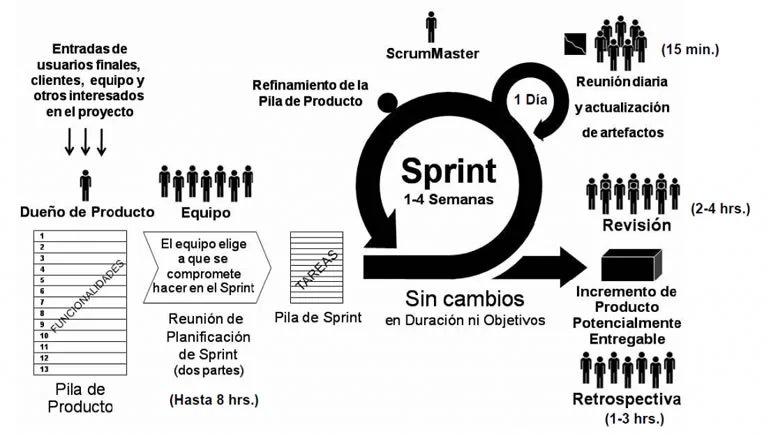
\includegraphics[width=0.85\textwidth]{imgs/scrum}
    \caption{Figura de una metodología SCRUM paradigmática}
    \label{fig:scrum}
\end{figure}

\paragraph{}A así, la planificación ha constado de cuatro ``sprints'' de cuatro cascadas
de aproximadamente de una  semana de duración cada uno.

\begin{figure}[H]
    \centering
    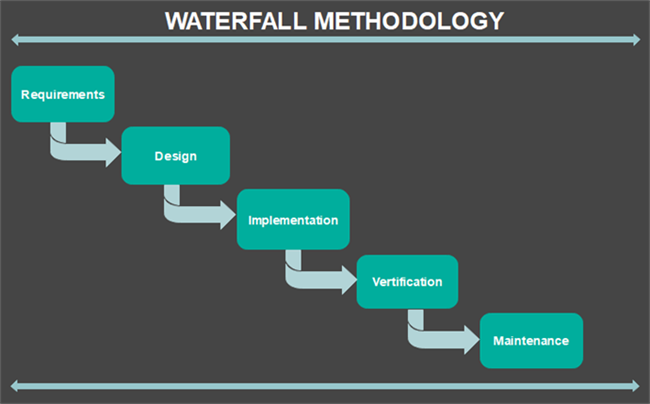
\includegraphics[width=0.85\textwidth]{imgs/waterfall}
    \caption{Figura de una metodología en cascada o \emph{waterfall}}
    \label{fig:waterfall}
\end{figure}

\subsection{Sprint 1: Entorno de desarrollo general.}

\paragraph{}Blabla

\subsection{Sprint 2: Aplicación Flutter.}

\paragraph{}Blabla

\subsection{Sprint 3: Yocto.}

\paragraph{}Blabla

\subsection{Sprint 4: Universalización y coherencia entre entornos.}

\paragraph{}Blabla

\section{Presupuesto}

\subsection{Personal}

\paragraph{} En este caso, el proyecto ha sido llevado a cabo por un sólo desarrollador.
Incluyendo la fase de planificación, diseño y desarrollo, la dedidación en horas ha sido
aproximadamente de un mes a media jornada (6 horas), además debemos tener en cuenta el
nivel de conocimientos trasnversales propios de un ingeniero senior.


\begin{table}[hbt]
	\label{t:recursoshumanos}
	\centering
	\begin{tabular}{|c|c|c|c|c|}
		\hline
        \textbf{Días trabajados} & \textbf{Horas al día} & \textbf{Total} & Precio [\euro/hora] & \textbf{Total} \\
		\hline
		22 & 6 & 132 & 15 & 1980 \\
		\hline
	\end{tabular}
	\caption{Desglose de horas dedicadas.}
\end{table}

\subsection{Material}

\paragraph{}Los materiales utilizados son una Raspberry Pi rev.3B+, una tarjeta microSD
de 16 Gb, un cable de alimentación, una fuente alimentación, una pantalla LCD 5" táctil,
y carcasa impresa en 3D.


\begin{table}[hbt]
	\label{t:materialescostes}
	\centering
	\begin{tabular}{|c|c|c|c|}
		\hline
		\textbf{Producto} & \textbf{Coste unidad [\euro]} & \textbf{Cantidad} & \textbf{Subtotal [\euro]} \\
		\hline
		Rbpi rev.3B+ & 37 & 1 & 37 \\
		\hline
		microSD & 10 & 1 & 10 \\
		\hline
        Alimentación & 15 & 1 & 15 \\
		\hline
        Pantalla LCD 5" & 20 & 1 & 20 \\
		\hline
        Carcasa 3D & 5 & 1 & 5 \\
		\hline
		\textbf{Total} & & & 87 \\
		\hline
	\end{tabular}
    \caption{Desglose de presupuesto de materiales.}
\end{table}

\subsection{Otros costes}

\paragraph{}Dentro de esta sección podremos considerar, por ejemplo:

\begin{itemize}
    \item Licencias de software.
    \item Suscripciones a servicios.
    \item Factura de la luz.
    \item Gastos de papelería.
    \item Etcetera.
\end{itemize}

Sin entrar en demasiado detalle podemos estimar una cantidad total para el total de los
conceptos descritos anteriormente de 30\euro.

\subsection{Resumen de costes}

\paragraph{}Teniendo en cuenta los costes desglosados en los apartados anteriores, el
presupuesto del proyecto queda de la siguiente manera:

\begin{table}[hbt]
	\label{t:resumencostes}
	\centering
	\begin{tabular}{|c|c|}
		\hline
		\textbf{Concepto} & \textbf{Gasto [\euro]} \\
		\hline
		Personal & 1980 \\
		\hline
		Material & 87 \\
		\hline
		Otros & 30 \\
		\hline
		\textbf{Total} & 2097 \\
		\hline
	\end{tabular}
    \caption{Resumen del presupuesto del proyecto.}
\end{table}

\paragraph{}Se puede considerar un proyecto de ingeniería barato ya que requiere de
muy pocos recursos y materiales y utiliza software de código abierto. Como suele ser
habitual en estos casos, el recurso más límitado y valioso son los recursos humanos.
Por eso, en el ámbito de las \glsplural{startup} es fundamental encontrar a gente
que tenga mucho que aportar y dar la oportunidad a becarios con mucha energía y ganas
de aprender.

\paragraph{}El presupuesto refleja el proyecto en un estado de \gls{MVP}. Es decir,
que es el coste de producir pocas unidades de prototipos funcionales que puedes mostrar
a \glsplural{early bird}. Y en base al feedback recogido, poder seguir buscando inversores,
mejorando la ingeniería del proyecto y llevando el producto a fase de producción.
